\documentclass{standalone}
\usepackage{tikz}
\usepackage{pgffor}
\usetikzlibrary{positioning}

\begin{document}
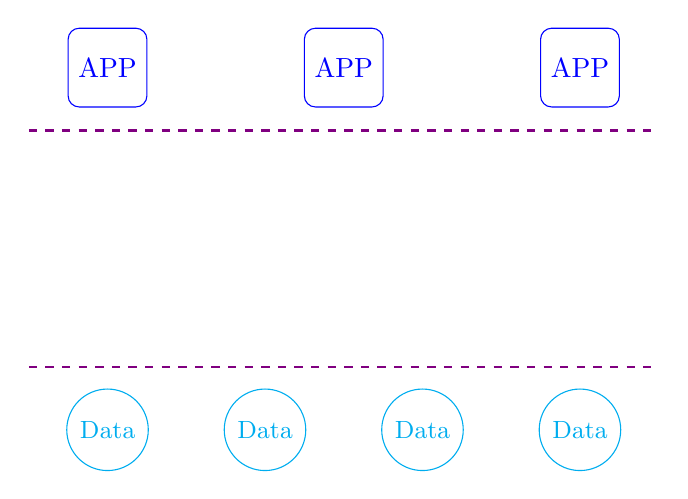
\begin{tikzpicture}[sep/.style = {dashed, thick, violet}, 
      app/.style = {draw, rectangle, minimum size = 1.0cm, blue, rounded corners},
      data/.style = {draw, circle, minimum size = 0.50cm, cyan, font = \small}]
  \def\len{8}
  \draw[sep] (0,0) to (\len,0);
  \draw[sep] (0,-3) to (\len,-3);

  \def\appy{0.8}
  \foreach \x in {1,4,7}
  \node[app] at (\x, \appy) {APP};

  \foreach \x in {1,3,5,7}
  \node[data] at (\x, -3.8) {Data};
\end{tikzpicture}
\end{document}